\documentclass[tikz,border=5mm]{standalone}
\usepackage{tikz}
\usetikzlibrary{arrows.meta,positioning}
\begin{document}
% Grafcet : A6_SFC
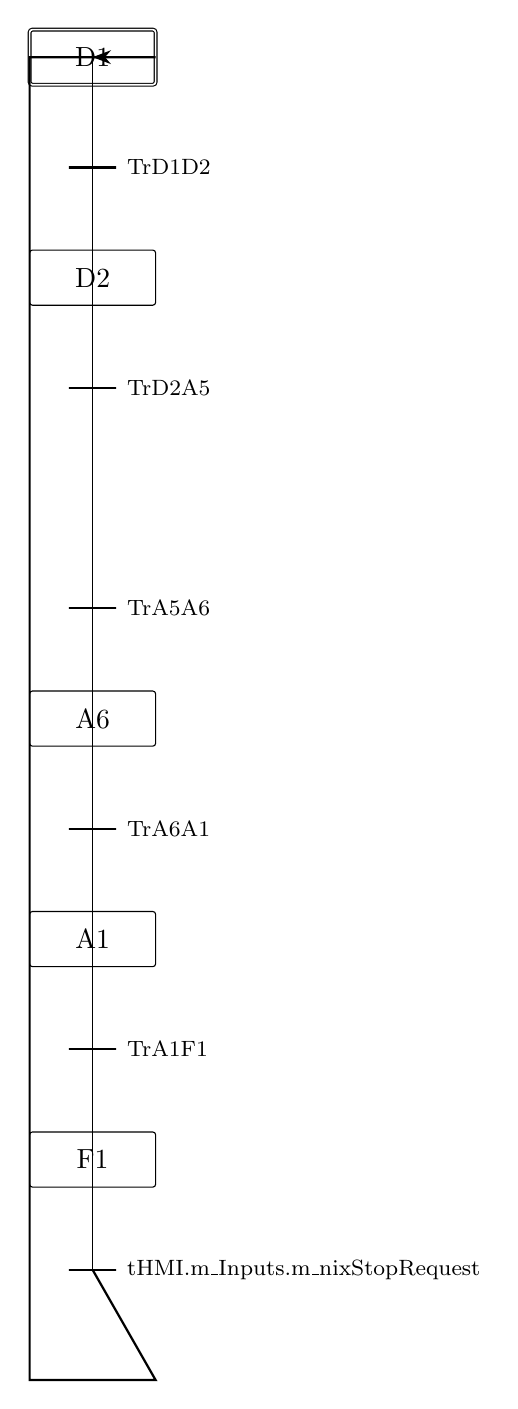
\begin{tikzpicture}[
  sfcstep/.style  = {draw, rounded corners=1pt, minimum width=16mm, minimum height=7mm, inner sep=1pt},
  sfcinit/.style  = {draw, double, rounded corners=1pt, minimum width=16mm, minimum height=7mm, inner sep=1pt},
  sfctrans/.style = {draw, line width=0.8pt, minimum width=6mm, minimum height=0pt, inner sep=0pt},
  sfcbranch/.style= {line width=1.4pt},
  sfclink/.style  = {->, >=Stealth, line width=0.8pt},
  x=16mm, y=-14mm,
]

  \node[sfcinit] (s196609) at (5.00,0.00) {D1};
  \node[sfcstep] (s196610) at (5.00,2.00) {D2};
  \node[sfcstep] (s196614) at (5.00,10.00) {F1};
  \node[sfcstep] (s196617) at (5.00,6.00) {A6};
  \node[sfcstep] (s196618) at (5.00,8.00) {A1};
  \node[sfctrans,label={right:\footnotesize TrD1D2}] (t0) at (5.00,1.00) {};
  \node[sfctrans,label={right:\footnotesize TrD2A5}] (t1) at (5.00,3.00) {};
  \node[sfctrans,label={right:\footnotesize TrA5A6}] (t2) at (5.00,5.00) {};
  \node[sfctrans,label={right:\footnotesize tHMI.m\_Inputs.m\_nixStopRequest}] (t3) at (5.00,11.00) {};
  \node[sfctrans,label={right:\footnotesize TrA6A1}] (t4) at (5.00,7.00) {};
  \node[sfctrans,label={right:\footnotesize TrA1F1}] (t5) at (5.00,9.00) {};
  \draw (5.00,0.00) -- (5.00,1.00);
  \draw (5.00,1.00) -- (5.00,2.00);
  \draw (5.00,2.00) -- (5.00,3.00);
  \draw (5.00,3.00) -- (5.00,5.00);
  \draw (5.00,5.00) -- (5.00,6.00);
  \draw (5.00,6.00) -- (5.00,7.00);
  \draw (5.00,7.00) -- (5.00,8.00);
  \draw (5.00,8.00) -- (5.00,9.00);
  \draw (5.00,9.00) -- (5.00,10.00);
  \draw (5.00,10.00) -- (5.00,11.00);
  \draw[sfclink] (5.00,11.00) -- (5.50,12.00) -- (4.50,12.00) -- (4.50,0.00) -- (5.50,0.00) -- (5.00,0.00);
\end{tikzpicture}
\end{document}
